\title{Big Data Applications in the Energy and Utilities Sector}


\author{Neha Rawat}
\affiliation{%
	\institution{Indiana University}
	\city{Bloomington} 
	\state{Indiana} 
}
\email{nrawat@iu.edu}



% The default list of authors is too long for headers}
\renewcommand{\shortauthors}{N. Rawat}


\begin{abstract}
	Efficient management and utilization of energy and other utilities is the need of the hour. The plethora of real-time data generated during day-to-day operational activities can be used to detect consumption patterns and predict outages, shortages and surges in power usage, while simultaneously improving the use of renewable resources as sustainable alternatives. Intelligent big data analytics can help the energy and utilities sector by reducing costs through devising efficient operational strategies, becoming more self-sufficient and productive in their performance and improving customer satisfaction and interaction by making valuable suggestions to the consumers on how to use their resources better. 
\end{abstract}

\keywords{i523, HID224, Smart Grids, Energy Disaggregation, Demand-Side Management, Sustainability, Water Management}

\maketitle

\section{Introduction}

Energy sources such as electricity and fossil fuels like coal and petroleum, along with renewable solar and wind energy, coupled with other utilities like water and gas, are indispensable entities for humans in their day-to-day processes. We can therefore imagine the pressure on the energy and utilities sector to provide uninterrupted resource flow while ensuring efficient management of those resources. Apart from this, sustainability and use of cleaner energy is also a demand upon these industries. In earlier times, the interaction used to be a one-way street, with the industries adjusting their supply capacities in order to meet demands of the consumers. With time, the demands have increased exponentially, and the supply needs to keep pace with it. This results in issues of demand management, operational inefficiencies and increasing strain on available resources. Therefore, the energy and utilities sector too has turned to Big Data analytics for a solution. The objectives are to design intelligent systems, using the wealth of data accumulated by the energy and utilities sector, which can assist in generating, storing and using energy sustainably to meet consumer needs, while keeping costs in check (cite1). New analytics systems designed for these purposes have the capability to actively store millions of records per second from  distributed sources, analyze these streams of events to detect patterns useful for prediction and constantly self-learn from previous responses using advanced cognitive capabilities (cite1).
\begin{figure}
	\includegraphics[width=\columnwidth]{images/"IBM EventStore".pdf}
	\caption{IBM's event-driven Data Management System (cite1)}
	\label{F:event}
\end{figure}
Figure \ref{F:event} shows how IBM's event-driven data management system works as an efficient analytics tool for the energy sector.\\
The advantages that these systems can provide utilities will be visible in form of cost reductions (increasing capital productivity and saving excess expenditures on operations and maintenance), increased reliability (predicting outages and accurately detecting failures of equipments) and customer satisfaction (engaging customers in the process flow by providing them with useful insights about their consumption patterns) (cite2). Some of these smart technologies have been actively deployed as well. GTM Research predicts that ``global utility company expenditure on data analytics will grow from 700 million in 2012 to 3.8 billion in 2020, with gas, electricity and water suppliers in all regions of the world increasing their investment'' (cite3).
   

\section{The Rise of Smart Technologies}
Big Data warehouses and analytic technologies have been making waves in the energy and utilities sector for some time now. One example is of Microsoft, where 30,000 existing sensors were organized into a single energy-efficient system, at the company's Redmond, Washington, headquarters (cite4). The network is used to avail billions of data points on energy usage in areas such as heating, cooling and lighting. Analysis of this data lead to, in one case, a garage exhaust fan, that had been running for a year and costing Microsoft 66,000 USD. Through this system, the company saves close to a ``60 million USD capital investment in energy-efficient technologies'' (cite4). On a larger scale, there is huge amount of data available, being generated from oil wells, electricity and other utility grids, and generation stations. Using big data technologies coupled with the Internet of Things (IoT) i.e. smart sensors, all of this information can be gathered, structured and analyzed to provide valuable insights on utility management.

\subsection{Smart Meters and Grids}
A {\em Smart Meter} differs from a regular meter in its additional abilities of not only measuring the energy consumption for the customer, but also processing it and providing real-time feedback regarding it. Some of the features of a smart meter are as follows:  real-time registration of energy usage, possibility to get meter information locally and remotely, remote access of the meter for adjustment of throughput, interconnection among various devices on the premise, ability to read other commodity meters in the vicinity (cite5).
\begin{figure}
	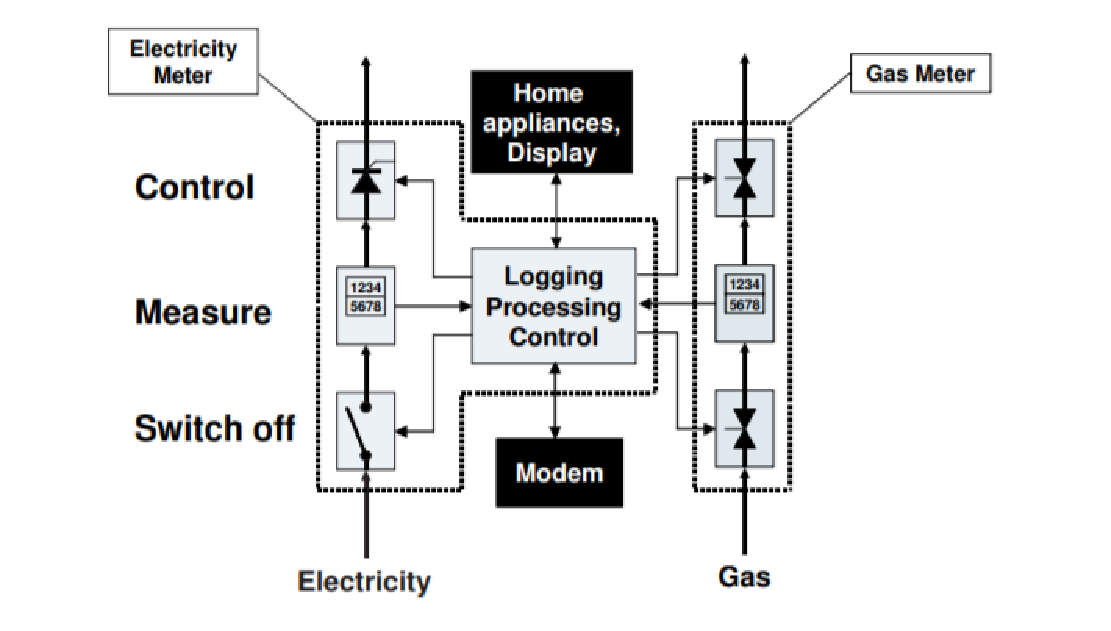
\includegraphics[width=\columnwidth]{images/smart_meter.pdf}
	\caption{Typical Smart Meter Structure (cite5)}
	\label{F:smart}
\end{figure}
Figure \ref{F:smart} shows a typical smart meter structure.\\
The {\em smartness} of a smart meter lies in its communication system. The meter can communicate using a Power Line Carrier, a wireless modem (GSM) or an existing internet connection. An interface can be used to connect this meter to appliances and a home display, using which it can show the energy data and costs to the consumer (cite5).\\
Though generally used for measuring energy consumption, smart meters can also be employed for other utilities such as gas and water. Smart water meters are not as common, but if implemented properly, can help detect issues such as leaks on the premises, in the main line, and wastage of water, much more promptly than with traditional technologies (cite9). Smart metering technologies, in general, can prove to be an essential addition to demand response as well as predictive management techniques.\\
A {\em Smart Grid} network is an advanced form of a traditional power grid (the concept is generally applied in the electricity sector). It provides a two-way exchange of electricity and information to create a widely distributed energy-delivery system, which is reliable, resilient and sustainable (cite6). Technologies such as smart meters act as components of a smart grid framework, which acts as an intelligent system that monitors generation, transmissions and consumption in the complete electric grid and performs dynamic energy management. For example, in case of a transformer failure, the smart grid would detect it and modify the power flow such that it recovers the power delivery service (cite6). Apart from this, smart grids can also be used in shaping energy demand profiles. The three major components in a smart grid system are: smart infrastructure, smart management and smart protection. The smart infrastructure helps in advanced energy flow, monitoring and communication. The smart management system provides control services. The smart protection system ensures reliability, safety and security of the network (cite6).
\begin{figure}
	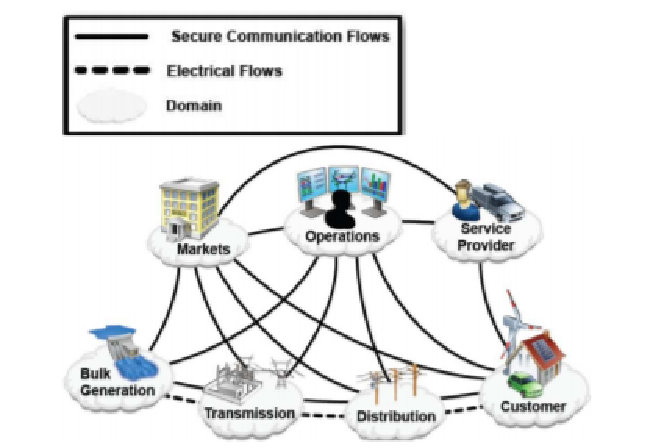
\includegraphics[width=\columnwidth]{images/smart_grid.pdf}
	\caption{Conceptual model for a Smart Grid (cite6)}
	\label{F:grid}
\end{figure}
Figure \ref{F:grid} shows the NIST conceptual model for a Smart Grid.\\
Thus, we see that the volume of data obtained from smart meters in smart grid networks, along with other components, can be used for a variety of intentions. For example, Diamantoulakis, Kapinas and Karagiannidis have used smart grid information for the purpose of load synchronization. Cloud computing technologies have been used to manage the big data obtained from a smart grid (using distributed data management and parallelization). Next, dimensionality reduction has been applied to keep only the useful predictors and data mining techniques like Artificial Neural Networks or Clustering have been used to model customer load curves. This has been followed by short-term load forecasting techniques (using regression, time-series or state-space models) to provide values for price and demand forecasts (cite7).
\begin{figure}
	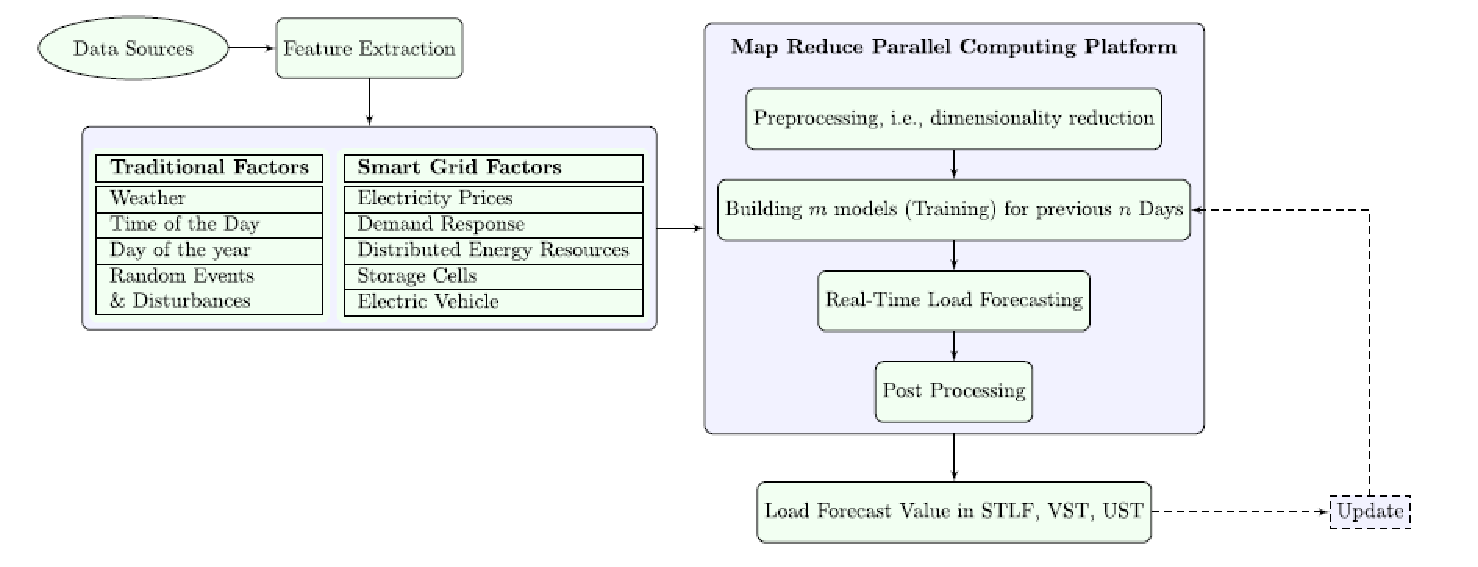
\includegraphics[width=\columnwidth]{images/sg_forecast.pdf}
	\caption{Smart Grid Forecast Model (cite7)}
	\label{F:forecast}
\end{figure}
Figure \ref{F:forecast} shows a rough structure of the Smart Grid forecast model.

\subsection{Energy Disaggregation}
{\em Energy Disaggregation} is a novel idea born out of the possibilities offered by the smart metering technologies discussed above. It involves the breakdown of the main electric signal into consumption by each individual appliance in a unit. Also referred to as NILM (Non-Intrusive Load Monitoring), this technology can help create itemized energy bills for consumers and help them monitor their consumption in a much more specific format. This in turn helps in efficient management of the power grid as well, as the user can detect if any device is faulty or consuming more than the normal amount of energy (cite8). The data generated by smart meters can be used for this process. The main electric signal can then be broken down into signals from individual appliances by identifying their signatures. This data obtained on an individual as well as aggregate level can be analyzed using data mining techniques such as deep learning (neural networks), Combinatorial Optimization or Factorial Hidden Markov Models (FHMM) to detect patterns useful for prediction purposes (cite8).

\subsection{Electric Vehicles}
The advent of {\em Electric vehicles} has largely reduced the strain on non-renewable fossil fuels. They form an important part of the Smart Grid network discussed in the previous section. The increase in use of electric vehicles leads to beneficial reduction in carbon emissions as well. However, one major consideration in the use of electric vehicles is charging these vehicles without overloading the grid (cite10). However, data analytics can help us here by designing scheduling systems for charging of these vehicles. Control mechanisms need to be set up to guide the charging of these vehicles. Also, consumers need to be explained to or incentivized so that they follow these guidelines and ensure that the load on the electric grid is stabilized. The advantage of electric vehicles is the presence of large batteries which can store charge and often help in load shifting within the owner's home. This indirectly provides energy back to the grid and helps stabilize it as well. Optimization techniques, using the data obtained from use of these vehicles (their charging-discharging cycles and energy demands), can help in devising such load scheduling systems which prove to be beneficial units of the Smart Grid system (cite10). 


\section{Growth Areas in the Energy Industry}
The advancement of technology has led to a cultural shift in the energy industry as well. Not only are technologies changing, but also the mindsets and therefore business strategies of companies in the energy sector (cite11). Some of the major areas in the industry touched by the advent of big data technologies are operations, asset management, demand-side management and customer satisfaction. Apart from these areas, the concept of sustainability is one of utmost importance. Efficient usage of renewable resources is another major benefit provided by data analytics to the energy industry.

\subsection{Asset Management and Operational Efficiency}



\section{Water Management}

\section{Case Studies}


\section{Conclusions}

\bibliographystyle{ACM-Reference-Format}
\bibliography{report}